\documentclass[11pt]{article}
\input{/Users/markwang/.preamble}
\begin{document}

\section{Multi-indices and higher order partials}

\subsection{Second-Order Partial Derivatives}


\begin{theorem}
  \label{Clairut's Theorem}
  \textbf{Clairut's Theorem} Let $f:\R^n \rightarrow \R$ be a function and $a\in\R^n$ a point. Let $i,j \in \{ 1, ..., n \}$  with $i\neq j$. If $\partial_{ij} f(a)$ and $\partial_{ji} f(a)$ both exist and are continuous in a neighbourhood of $a$, then $\partial_{ij} f(a) = \partial_{ji} f(a)$
\end{theorem}

\begin{defn}
  \label{C2 functions} \textbf{$C^2$ Functions} Let $U\in\R^n$ be an open set. We define $C^2(U, \R)$ to be the collection of $f:\R^n \rightarrow \R$ whose second partial derivatives exist and are continuous at every point in $U$

  \begin{rem}
    Therefore, if $f$ is a $C^2$ function, Clairut's theorem immediately imply that it's mixed partials exists, continuous, and hence are equal.
  \end{rem}
\end{defn}

$ $\\
An example in using high-order partial derivatives in conjunction with the chain rule.
Let $u=f(x,y)$ and suppose $x,y$ are functions of $(s,t)$, i.e. $x(s,t)$, $y(s,t)$. Compute $\frac{\partial^2 y}{\partial s^2}$
\begin{solution}
  $ $\\
  Using the chain rule we have first order partials
  \[
    \frac{\partial u}{\partial s} = \frac{\partial u}{\partial x}\frac{\partial x}{\partial s} + \frac{\partial u}{\partial y}\frac{\partial y}{\partial s}
  \]
  Then we take partials again with respect to $s$
  \[
    \frac{\partial^2 u}{\partial s^2} = \frac{\partial}{\partial s}\left[\frac{\partial u}{\partial s}\right] = \frac{\partial}{\partial s} \left[\frac{\partial u}{\partial x}\frac{\partial x}{\partial s}\right] + \frac{\partial}{\partial s} \left[\frac{\partial u}{\partial y}\frac{\partial y}{\partial s}\right]
  \]
  Note here $\frac{\partial u}{\partial s}$ is a function of $(x,y)$. Thus to differentiate this function with respect to $s$, we must once again use the chain rule.
  \begin{align*}
    \frac{\partial}{\partial s}\left[ \frac{\partial u}{\partial x}\frac{\partial x}{\partial s}\right] &= \left[ \frac{\partial}{\partial s}\frac{\partial u}{\partial x}\right]\frac{\partial x}{\partial s} + \frac{\partial u}{\partial x}\frac{\partial^2 x}{\partial s^2} \tag{\text{product rule}}\\
    &= \left[ \frac{\partial^2 u}{\partial x^2} \frac{\partial x}{\partial s} + \frac{\partial^2 u}{\partial x \partial y}\frac{\partial y}{\partial s} \right] \frac{\partial x}{\partial s} + \frac{\partial u}{\partial x}\frac{\partial^2 x}{\partial s^2} \tag{\text{chain rule}}\\
    &= \frac{\partial^2 u}{\partial x^2} \left[ \frac{\partial x}{\partial s} \right]^2 + \frac{\partial^2 u}{\partial x \partial y}\frac{\partial y}{\partial s}\frac{\partial x}{\partial s} + \frac{\partial u}{\partial x}\frac{\partial^2 x}{\partial s^2}\\
  \end{align*}
  Similar computation can be applied to the latter term. Then
  \[
    \frac{\partial^2 u}{\partial s^2} =  \frac{\partial^2 u}{\partial x^2} \left[ \frac{\partial x}{\partial s} \right]^2 + \frac{\partial^2 u}{\partial y^2} \left[ \frac{\partial y}{\partial s} \right]^2 + 2 \frac{\partial^2 u}{\partial x \partial y} \frac{\partial y}{\partial s}\frac{\partial x}{\partial s} + \frac{\partial u}{\partial x}\frac{\partial^2 x}{\partial s^2} + \frac{\partial u}{\partial y}\frac{\partial^2 y}{\partial s^2}
  \]
\end{solution}

  \begin{defn}
    \label{Higher Order Partials}\textbf{Higher Order Partials} If $U\subseteq \R^n$ is an open set, then for $k\in\N$ we define $C^k(U, \R)$ to be the collection of functions $f:\R^n \rightarrow \R$ such that the $k$-th order partial derivatives of $f$ all exist and are continuous on $U$. If the partials exist and are continuous for all $k$, we say that $f$ is of type $C^{\infty}(U, \R)$
  \end{defn}

  \begin{theorem}
    \label{Generalized Clairuit's Theorem} \textbf{Generalized Clairuit's Theorem} If $f:U\subseteq \R^2 \rightarrow \R$ is of type $C^k$, then
    \[
      \partial_{i_1 \dots i_k} f = \partial_{j_1\dots j_k} f
    \]
    whenever $(i_1, \dots, i_k)$ and $(j_1, \dots, j_k)$ are re-orderings of each other.
  \end{theorem}


  \begin{defn}
    \label{Multi-indices}\textbf{Multi-index notation}
    A multi-index $\alpha$ is a tuple of non-negative integers
    \[
      \alpha = (\alpha_1, \dots, \alpha_n)
    \]
    The \textbf{order}  of $\alpha$ is the sum of its components
    \[
      | \alpha | = \alpha_1 + \alpha_2 + \dots + \alpha_n
    \]
    We define the multi-index \textbf{factorial} to be
    \[
      \alpha ! = \alpha_1 ! \alpha_2 ! \dots \alpha_n !
    \]
    If $x = (x_1, \dots, x_n)\in\R^n$ then the multi-index \textbf{exponential} is
    \[
      x^{\alpha} = x_1^{\alpha_1} x_2^{\alpha_2} \dots x_n^{\alpha_n}
    \]
    and if $f:\R^n \rightarrow \R$ we write
    \[
      \partial^{\alpha} = \frac{\partial^{| \alpha |} f}{\partial x_1^{\alpha_1} \partial x_2^{\alpha_2} \dots \partial x_n^{\alpha_n}}
    \]
  \end{defn}

  \section{Taylor Series}

  \subsection{review}

  Derivatives can be a tool for linearly approximating a function
  \[
    f(x) \approx f(a) + f'(a)(x-a)
  \]
  \\We can go beyong just linear approximation and introduce quadratic, cubic, quartic approximations.
  \[
    p_{n,a} (x) = \sum_{k=0}^{n} c_k (x-a)^k \text{ , where } c_k = \frac{f^{(k)}(a)}{k!}
  \]
  Note here $p$ is an expansion of $f$
  \[
    T_n(x) = p_{n,a}(x) = \sum_{k=0}^{n} \frac{f^{(k)}(a)}{k!} (x-a)^k
  \]
  is a taylor polynomial of $f$ of degree $n$ with center $a$


\begin{theorem*}
  Let a function $f$ be $C^{\infty}$, let $T$ be the Taylor polynomial of $f$ of degree $n$ with center $a$. Then for all $k\in [0, n]$,
  \[
    T^{(k)}(a) = f^{(k)}(a)
  \]
\end{theorem*}


\begin{defn*}
  \label{One-Var Taylor Series} \textbf{Single variable Taylor's Theorem} Let $f: [a,b]\subseteq \R \rightarrow \R$. Let $n>0$ $n\in \mathbb{Z}$. Suppose $f^{(n)}$ is continuous on $[a,b]$ and $f^{(n+1)}(x)$ exists on $(a,b)$. Let $\alpha, \beta \in [a,b]$. Then Taylor polynomial of degree $n$ of function $f$ at point $x$, is denoted as
  \[
    p(x) = p_{n, \alpha} = \sum_{k=0}^{n} C_k (t-\alpha)^k, \text{ , where } C_k = \frac{f^{(k)}(\alpha)}{k!} \in\R
  \]
  \begin{rem}
    Here $p(x)$ and $f(x)$ have derivatives at $\alpha$ that agree up to order $n$; that is
    \[
      \forall k\in \{1,\dots, n\}: p^{(k)}(\alpha) = f^{(k)}(\alpha)
    \]
    Also note that
    \[
      f(x) = p_{n, \alpha}(x) + r_{n, \alpha} (x)
    \]
  \end{rem}
  \noindent If $f$ is defined above, then for each $\beta$ there eists a point $c$ between $\alpha,\beta$ such that

   \[
    f(\beta) = p_{n, \alpha}(\beta) + \frac{f^{(n+1)}(c)}{(n+1)!} (\beta - \alpha)^{n+1}
   \]

  \begin{figure}[h!]
    \centering
    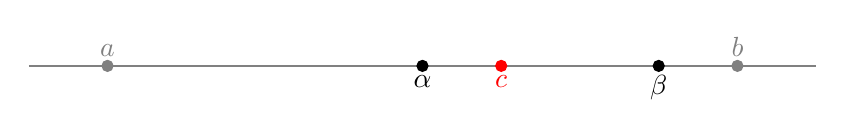
\begin{tikzpicture}
      \draw[gray, thick] (-5,0) -- (5,0);
      \filldraw[black] (0,0) circle (2pt) node[anchor=north] {$\alpha$};
      \filldraw[black] (3,0) circle (2pt) node[anchor=north] {$\beta$};
      \filldraw[red] (1,0) circle (2pt) node[anchor=north] {$c$};
      \filldraw[gray] (-4,0) circle (2pt) node[anchor=south] {$a$};
      \filldraw[gray] (4,0) circle (2pt) node[anchor=south] {$b$};
    \end{tikzpicture}
  \end{figure}

\end{defn*}



\begin{theorem*}
  \textbf{Rolle's Theorem} If a real-valued function $f$ is continuous on a proper closed interval $[a, b]$, differentiable on the open interval $(a, b)$, and $f(a) = f(b)$, then there exists at least one $c$ in the open interval $(a, b)$ such that
  \[
    f'(c) = 0
  \]
  \begin{proof}
    Since $[a, b]$ closed and bounded, intermediate value theorem applies here; that is, $f(x)$ achieves its maximum and minimum over $[a,b]$. Let $c\in[a,b]$. If $c\in(a,b)$, since $f$ is differentiable on $(a,b)$, $f'(c) = 0$ because it is an extremum. If $c\in \{ a, b\}$ or maximum and minimum occurs at endpoints. Because $f(a) = f(b)$, then it means that $f(x)$ cannot be greater or smaller than $f(a) = f(b)$, then $f(x)$ is a constant function and $f'(x)$ is therefore 0 over $(a,b)$
  \end{proof}
  \begin{rem}
    Rolle's Theorem is used to prove the Mean Value Theorem. We will prove this here
  \end{rem}
  \begin{proof}
    Let $f: \R \to \R$ be continuous on $[a,b]$ and differentiable on $(a,b)$. Define
    \[
      g(x) = f(x) - rx
    \]
    for some $r\in \R$. Now we want to choose $r$ so that $g(x)$ satisfies Rolle's Theorem, specifically,
    \[
      g(a) = g(b) \iff f(a) - ra = f(b) - rb \iff r = \frac{f(b) - f(a)}{b-a}
    \]
    By Rolle's theorem since $g(x)$ is differentiable and $g(a) = g(b)$, then there exists $c\in (a,b)$ for which $g'(c) = 0$, i.e.,
    \[
      g'(c) = f'(c) - r \iff f'(c) = g'(c) + r = \frac{f(b) - f(a)}{b-a}
    \]
  \end{proof}

\end{theorem*}


\begin{theorem*}
  \label{Higher Order Rolle's Theorem} \textbf{Higher Order Rolle's Theorem} Assume that $f: \R \rightarrow \R$ is continuous on $[a,b]$ and $n+1$ times differentiable on $[a,b]$. If $f(a) = f(b)$ and $f^{(k)}(a) = 0$ for all $k\in \{ 1, \dots, n\}$ then there exists a $c\in (a,b)$ such that $f^{(n+1)}(c) = 0$
  \begin{proof}
    Note that $f^{(k)}(a) = 0$ for all $k\in \{ 1, \cdots, n\}$ while no such constraint on the other endpoint $b$. All condition of Rolle's Theorem apply here with $f(a) = f(b)$, so there exists $\theta_1 \in (a,b)$ such that $f'(\theta_1) = 0$. Again with $f'(a) = f'(\theta_1) = 0$, there exists $\theta_2 \in (a, \theta_1)$ such that $f''(\theta_2) = 0$. We can continue inductively in this fashion until $f^{(n)}(a) = f^{(n)}(\theta_n)$, so that there exists $c := \theta_{n+1} \in (a, \theta_n) \subseteq (a,b)$ such that $f^{(n+1)}(c) = 0$ as required
  \end{proof}
\end{theorem*}

\begin{theorem*}
  \label{Taylor's Theorem with Lagrange Reminder} \textbf{Taylor's Theorem with Lagrange Reminder} Suppose that $f$ is $n+1$ times differentiable on an interval $I$ with $a\in I$. For each $x\in I$ there is a point $c$ between $a$ and $x$ such that
  \[
    r_{n,a}(x) = \frac{f^{(n+1)}(c)}{(n+1)!} (x-a)^{n+1}
  \]
  so if $f$ is $k$ times differentiable at the point $a$, then
  \[
    f(x) = p_{n, a}(x) + r_{n, a}(x) = \sum_{k=0}^{n} \frac{f^{(k)}(a)}{k!} (x-a)^k + \frac{f^{(n+1)}(c)}{(n+1)!} (x-a)^{n+1}
  \]
\end{theorem*}

\begin{corollary*}
  \textbf{Taylor reminder is a good approximation} If $f$ is of type $C^{n+1}$ on an open interval $I$ with $a\in I$, then
  \[
  \lim_{x\to a} \frac{r_{n, a}(x)}{| x-a |^n} = 0
  \]

  \begin{proof}
    Since $f$ is of type $C^{n+1}$ we know that $f^{(n+1)}$ is continuous on $I$. Since $I$ is open and $a\in I$. We can find a closed inteval $J$ such that $a\in J\subseteq I$. Therefore $J$ is bounded. By Extreme Value Theorem, there exists $M > 0$ such that $|f^{(n+1)} (x)| \leq M$ for all $x\in J$. Since $f$ is $n+1$ times differentiable in $a$. We can construct Taylor polynomial with Lagrange reminder
    \begin{align*}
      \lim_{x\to a} \frac{|r_{n, a}(x)|}{|x-a|^n}  &= \lim_{x\to a} \frac{|f^{(n+1)}(c)|}{(n+1)!} \frac{|x-a|^{n+1}}{|x-a|^n} \\
      &= \lim_{x\to a} \frac{M}{(n+1)!} |x-a| \\
      &= 0
    \end{align*}
    Then by Squeeze theorem, $\lim_{x\to a} \frac{r_{n, a}(x)}{|x-a|^n} = 0$
    Moreover, we could bound $r_{n, a}(x)$ as
    \[
      | r_{n,a}(x) | \leq \frac{M}{(n+1)!} | x-a |^{n+1} \text{ , for some } M>0
    \]
  \end{proof}
  \begin{rem}
    This corollary just shows that the Taylor reminder is a good approximation, since error vanishes faster than order $n$. Also we can determine error bounds on Taylor series with the last formula since $f$ attains its maximum by Extreme Value Theorem.
  \end{rem}

\end{corollary*}


\begin{theorem}
  \label{Multi-variable Taylor's Theorem} \textbf{Multi-variable Taylor's Theorem} Let $f:\R^n \rightarrow \R$ where $f\in C^{k+1}(S, \R)$ where $S\subseteq \R^n$ be an open and convex set. Let $a = (a^1, \dots, a^n)\in S$ and $x = (x^1,\dots, x^n) \in S$. Then multivariate Taylor polynomial is given by
  \[
    f(x) = \sum_{|\alpha|\leq n} \frac{( \partial^{\alpha} f ) (a)}{\alpha !} (x-a)^{\alpha} + r_{n,a} (x) \text{ where } r_{n,a}(x) = \sum_{|\alpha| = n+1} \frac{\partial^{\alpha} f(c)}{\alpha!} (x-a)^{\alpha}
  \]
  Or consider $h = x - a$, then
  \[
    f(a+h) = \sum_{|\alpha|\leq n} \frac{( \partial^{\alpha} f ) (a)}{\alpha !} h^{\alpha} + \sum_{|\alpha| = n+1} \frac{\partial^{\alpha} f(c)}{\alpha !} h^{\alpha}
  \]
  for some $c$ on the line joining $a$ to $x$, i.e. there exists $t\in [0,1]$ such that
  \[
    c = a(1-t) + tx = a + t(x-a)
  \]
  \begin{rem}
    Taylor polynomials are \textit{unique}; that is if we ahve an order $k$ polynomial approximation to a function whose error vanishes in order $k+1$, then that polynomial is necessarily Taylor polynomial. This implies that the Taylor series of any polynomial is that polynomial itself.
  \end{rem}
\end{theorem}

\begin{defn*}
  Here is a list of common taylor series
  \begin{enumerate}
    \item
    \[
      \frac{1}{1-x} = 1 + x + x^2 + x^3 + \cdots = \sum_{k=0}^{\infty} x^k
    \]
    \item
    \[
      e^x = 1 + x + \frac{x^2}{2} + \frac{x^3}{3!} + \cdots = \sum_{k=0}^{\infty} \frac{x^k}{k!}
    \]
    \item
    \[
      sin(x) = x - \frac{x^3}{3!} + \frac{x^5}{5!} + \cdots = \sum_{k=0}^{\infty} = \frac{(-1)^kx^{2k+1}}{(2k+1)!}
    \]
    \item
    \[
      cos(x) = 1 - \frac{x^2}{2!} + \frac{x^4}{4!} - \frac{x^6}{6!} + \cdots = \sum_{k=0}^{\infty}(-1)^{k} \frac{x^{2k}}{(2k)!}
    \]
    \item
    \[
      \ln (1+x) = x - \frac{x^2}{2} + \frac{x^3}{3} - \frac{x^4}{4} + \cdots = \sum_{k=1}^{\infty} (-1)^{k+1} \frac{x^k}{k}
    \]

  \end{enumerate}
\end{defn*}


\subsection{The Hessian Matrix}

\begin{defn}
  \label{Hessian Matrix}\textbf{Hessian Matrix} If $f:\R^n \rightarrow \R$ is of class $C^2$ then the Hessian matrix of $f$ at $a\in\R^n$ is the symmetric (i.e. $H = H^T$) $n\times n$ matrix of second order partial derivatives
  \[
    H(a) =
    \begin{bmatrix}
      \partial_{11}f(a) & \partial_{12} f(a) & \dots  & \partial_{1n} f(a) \\
      \partial_{21}f(a) & \partial_{22} f(a) & \dots  & \partial_{2n} f(a) \\
      \vdots & \vdots & \ddots & \vdots \\
      \partial_{n1} f(a) & \partial_{n2} f(a) & \dots  & \partial_{nn} f(a)
    \end{bmatrix}
  \]
  \begin{rem}
    We can use notion of Hessian matrix to simplify Taylor series formula. For first term of polynomial expansion
    \[
      \sum_{|\alpha|=1}^{\infty} \frac{1}{\alpha!}(\partial^{\alpha}f)(a) (x_0 - a)^{\alpha} = \nabla f(a) \dot (x_0 - a)
    \]
    For second order polynomial expansion
    \[
      \sum_{|\alpha|=2}^{\infty} \frac{2}{\alpha!}(\partial^{\alpha}f)(a) (x_0 - a)^{\alpha} = (x_0-a)^T H(a) (x_0-a)
    \]
    So second-order Taylor polynomial is just
    \[
      f(x_0) = f(a) + \nabla f(a) (x_0-a) + \frac{1}{2} (x_0-a)^T H(a) (x_0-a) + r_{2, a} (x_0)
    \]
  \end{rem}
  Now we can compute simple Taylor polynomial not only from formula given but also from gradient and Hessian matrix.
\end{defn}

\begin{theorem}
  \label{Spectral Theorem} \textbf{Spectral Theorem} If $A: \R^n \rightarrow \R^n$ is a symmetric matrix then there exists an orthonormal basis consisting of eigenvectors of $A$. And all of its eigenvalues are real numbers. That is, there exists real numbers $\lambda_1 \leq \lambda_2 \leq \cdots \leq \lambda_n$, and vectors $v_1, \cdots, v_n$, such that
  \[
    Av_i =  \lambda_i v_i
  \]
  and
  \[
    v_i \cdot v_j =
    \begin{cases}
      1 & \text{ if } i = j \\
      0 & \text{ if } i\neq j
    \end{cases}
  \]
\end{theorem}






\end{document}
